A lot of work has been done in this field, resulting in many different prefetching heuristics. They
range from the very simple sequential ones, that simply fetches the address after the current one,
to more complex ones that tries to find patterns and use dynamically gathered statistics to guide
them \cite{prefetch_range}.

\subsection{Reference Prediction Tables}
Reference Prediction Tables (RPT) \cite{rpt} is a prefetching technique which uses a large table to
store information indexed by the program counter of the load. It calculates the delta for each miss,
but the prefetching is only done after a certain amount of misses with the delta has occurred.

\subsection{Program Counter/Delta Correlation Prefetching}
Program Counter/Delta Correlation Prefetching (PC/DC) \cite{prefetch_range} is a prefetching method
using a Global History Buffer (GHB). It uses buffered delta calculations to search for stride
patterns. If a pattern is found, it is used to start prefetching.

\subsection{Delta Correlation Prediction Tables} 
Delta Correlation Prediction Tables combines RPT and PC/DC \cite{dcpt}. A large table is indexed by the program counter and Fig.~\ref{fig:dcpt_entry} shows an
entry in the table.
\begin{figure}[h]
	\begin{center}
		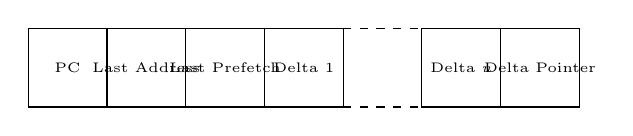
\begin{tikzpicture}
			\draw (0,0) rectangle (1,1);
			\draw (1,0) rectangle (2,1);
			\draw (2,0) rectangle (3,1);
			\draw (3,0) rectangle (4,1);
			\draw[dashed] (4,0) -- (5,0);
			\draw[dashed] (4,1) -- (5,1);
			\draw (5,0) rectangle (6,1);
			\draw (6,0) rectangle (7,1);

			\draw (0.5,0.5) node {\tiny PC};
			\draw (1.5,0.5) node {\tiny Last Address};	
			\draw (2.5,0.5) node {\tiny Last Prefetch};
			\draw (3.5,0.5) node {\tiny Delta 1};
			\draw (5.5,0.5) node {\tiny Delta \emph{n}};
			\draw (6.5,0.5) node {\tiny Delta Pointer};
		\end{tikzpicture}
	\end{center}
	\caption{DCPT entry\label{fig:dcpt_entry}}
\end{figure}
The \emph{PC} field contains the program counter of the load instruction. \emph{Last address}
contains the load address. The \emph{delta} fields contains the calculated delta values for this
load instruction. These delta fields works as a circular buffer, where the \emph{delta pointer}
field points to the head of the buffer. \emph{Last prefetch} stores the last prefetch address. 

When a new delta is calculated, it is stored in the circular buffer and the prefetcher goes through
the buffer to search for a match for the two newest calculated deltas. When a match is found the
first prefetch candidate is calculated by adding the delta after the match to the address in the
\emph{last address} field. The second one is calculated by adding the next delta value to the first
prefetch candidate. This is done for all the delta values after the matched pair, also with the
newest calculated delta values.
